\chapter{Introduction}
\label{chap:context}
In this dissertation I present SFL-explorer, a tool to help build intuitive understanding of how functional programming languages work. The ultimate goal of this project was to make a tool that makes learning and teaching the basics of functional programming easier. 

The two groups of stakeholders that I identified for this project are:
\begin{itemize}
  \item Those involved in teaching functional languages, as part of a university course or otherwise. They could such a tool to demonstrates functional languages to facilitate intuitive explanations in lectures.
  \item Those involved in learning functional languages. These could be students of a university course, or anyone interested in the topic. They could use such a tool to experiment with functional languages. 
\end{itemize}

% a tool to demonstrate how functional programming languages are evaluated, and help build intuitive understanding of how functional programming languages work. 
SFL-explorer takes the form of a functional language (\ac{SFL}), packaged with a web based interface that allows users to observe the process of evaluating a term as a series of step by step reductions, and control the order that sub-terms are evaluated.  It is an open source web based tool, available for download and offline use. A build of SFL explorer is submitted in the auxiliary materials, and it is also available at \href{https://functional.kiransturt.co.uk}{https://functional.kiransturt.co.uk}.

\section{The Language}
The language itself is not meant to be the main interest for the users of this system. It is designed to be fairly generic, with syntax and semantics similar to popular functional languages, so that users can take their understanding from using SFL-explorer and apply it to these languages. \ref{tab:fac_2_table_input} is an example program in the language, to find the factorial of 2. The relevant prelude functions are included for clarity.

\begin{figure}[h]
\begin{lstlisting}[language=SFL]
if :: Bool -> a -> a -> a
if cond then_branch else_branch = match cond {
  | true -> then_branch
  | false -> else_branch
}

fac :: Int -> Int
fac n = if (n <= 1) (1) (n * (fac (n - 1)))

main :: Int
main = fac 2
\end{lstlisting}
\caption{An example SFL program. Evaluation is shown \ref{tab:fac_2_table}}
\label{tab:fac_2_table_input}
\end{figure}

\ref{tab:fac_2_table} is a table showing the evaluation of this function in lazy mode by the system. The `Prompt' column shows what the user is presented with as a button to make progress. The first prompt entry at row $0$ is empty, as it represents the starting program state. This table is generated dynamically as the user progresses through the given program.  


\begin{figure}[t]
    \centering
    \begin{tabular}{|l|p{5cm}|l|}
\hline
    Step & \textbf{Prompt} & \textbf{Main Expression Afterwards} \\ \hline
    0 &     \  & \begin{lstlisting}[language=SFL_unboxed]
fac 2
\end{lstlisting}\rule[-2ex]{0pt}{0pt} \\ \hline
     1 & Apply function `fac' to 2 & \begin{lstlisting}[language=SFL_unboxed]
if (2 <= 1) 1 (2 * (fac (2 - 1)))
\end{lstlisting}\rule[-2ex]{0pt}{0pt} \\ \hline
    2 &\makecell[l]{Apply function if to (2 <= 1), 1 \\\ \ and (2 * (fac (2 - 1)))}
    & \begin{lstlisting}[language=SFL_unboxed]
match (2 <= 1) {
  | true -> 1
  | false -> 2 * (fac (2 - 1))
}
\end{lstlisting} \\\hline
    3 & Apply inbuilt <= to `2' and `1'  & \begin{lstlisting}[language=SFL_unboxed]
match (false) {
  | true -> 1
  | false -> 2 * (fac (2 - 1))
}
\end{lstlisting} \\\hline
     4 & Match to pattern `false' & \begin{lstlisting}[language=SFL_unboxed]
2 * (fac (2 - 1))
\end{lstlisting}\rule[-2ex]{0pt}{0pt} \\\hline
    5  & \makecell[l]{Apply function fac to (2 - 1)}
    & \begin{lstlisting}[language=SFL_unboxed]
2 * (if ((2 - 1) <= 1) 1 ((2 - 1) 
    * (fac ((2 - 1) - 1))))
\end{lstlisting} \\\hline
     
    6 & \makecell[l]{Apply function if to \\\ \ ((2 - 1) <= 1), 1 and \\\ \ ((2 - 1) * (fac ((2 - 1) - 1)))}
    & \begin{lstlisting}[language=SFL_unboxed]
2 * match ((2 - 1) <= 1) {
  | true -> 1
  | false -> (2 - 1) * (fac ((2 - 1) - 1))
}
\end{lstlisting} \\\hline
     
     7  & \makecell[l]{Apply inbuilt - to 2 and 1}
    & \begin{lstlisting}[language=SFL_unboxed]
2 * match (1 <= 1) {
  | true -> 1
  | false -> 1 * (fac (1 - 1))
}
\end{lstlisting} \\\hline

  8  & \makecell[l]{Apply inbuilt <= to 1 and 1}
    & \begin{lstlisting}[language=SFL_unboxed]
2 * match (true) {
  | true -> 1
  | false -> 1 * (fac (1 - 1))
}
\end{lstlisting} \\\hline
     
     9 & \makecell[l]{Match to pattern true}
    & \begin{lstlisting}[language=SFL_unboxed,aboveskip=0pt,belowskip=0pt]
2 * 1
\end{lstlisting}\rule[-2ex]{0pt}{0pt} \\\hline

   10 & \makecell[l]{Apply inbuilt $*$ to 2 and 1}
    & \begin{lstlisting}[language=SFL_unboxed,aboveskip=0pt,belowskip=10pt]
2
\end{lstlisting}\rule[-2ex]{0pt}{0pt}\\\hline
\end{tabular}
    \caption{A table showing how the system leads a user through the step by step evaluation of the program shown in Figure \ref{tab:fac_2_table_input}}
    \label{tab:fac_2_table}
\end{figure}

The user is provided with messages telling them what the next step that they can make is. Additionally, there is a `free choice' mode where users are presented with the options for progress, and they can choose which one is taken.

\section{Development Lifecycle}
\begin{figure}[t]
  \centering
  \fbox{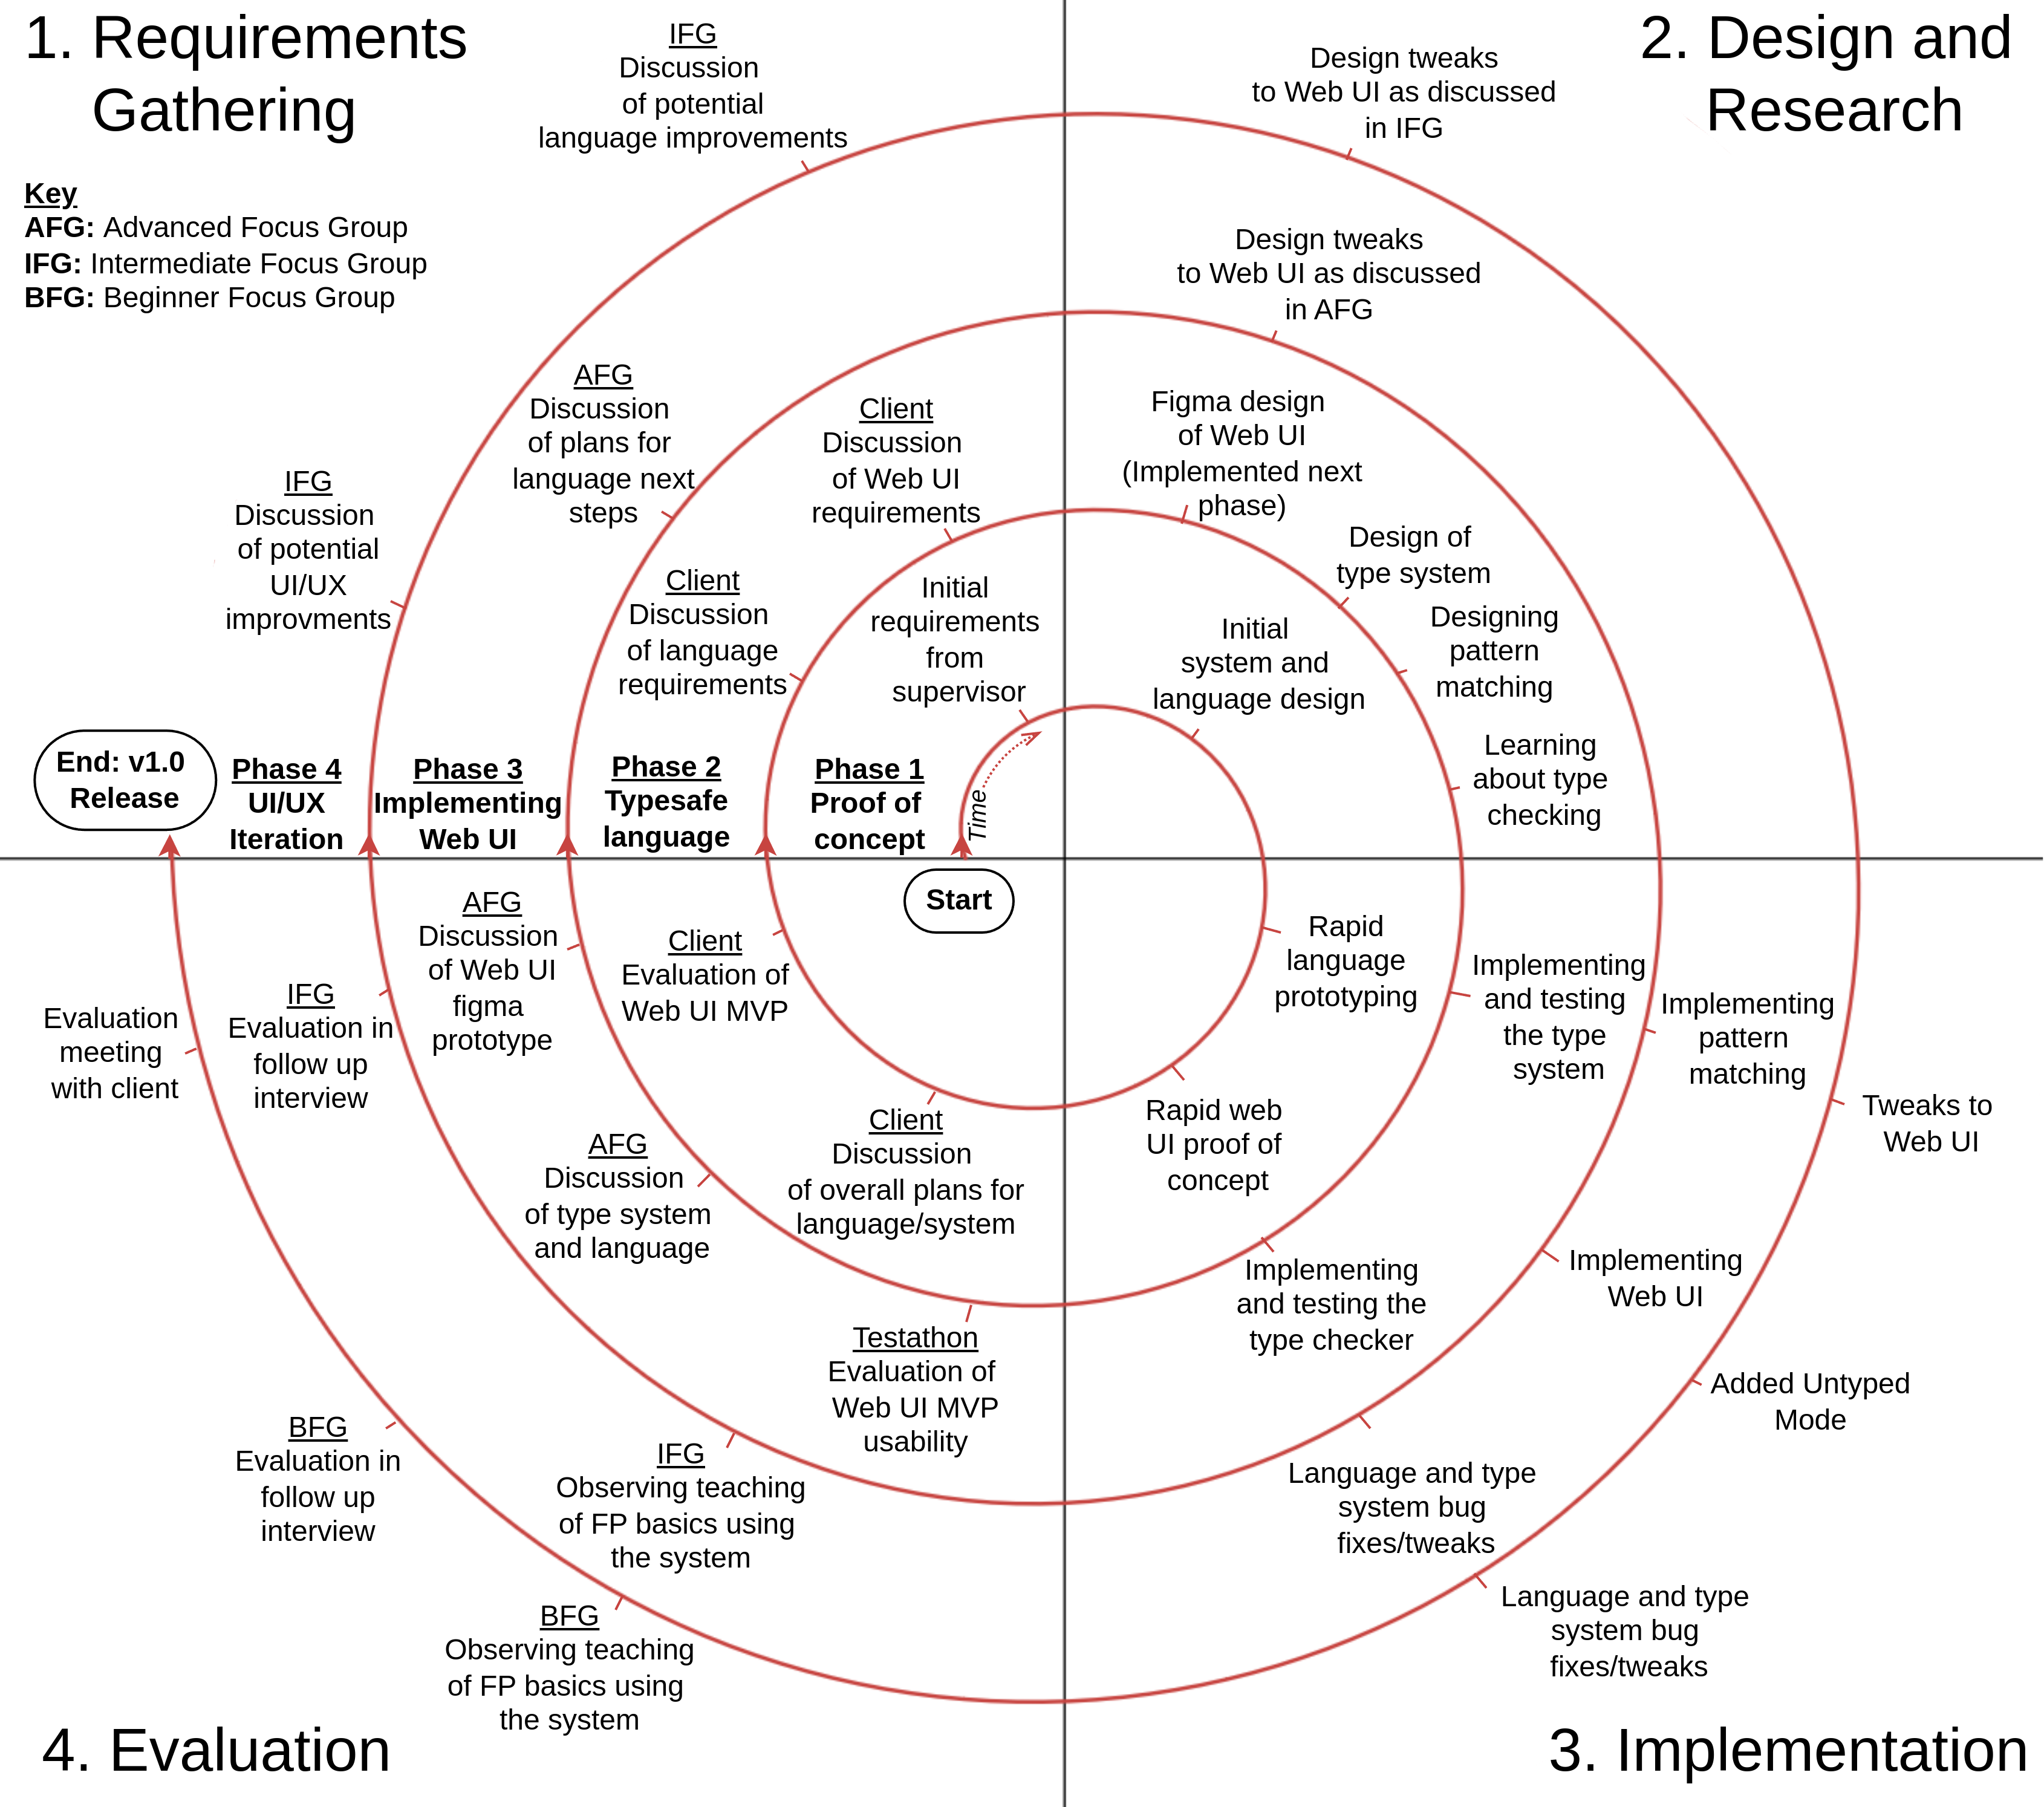
\includegraphics[width=0.98\linewidth]{images/spiral1-5.png}}
  \caption{A spiral representation of the project lifecycle, showing the 4 iterations, and the work done in each part of each phase. }\label{fig:spiral}
\end{figure}


The project followed a development lifecycle inspired by Agile principles~\cite{agilemanifesto2001}, structured into four iterative phases. 
Each phase was further subdivided into four phases: \textbf{Requirements Gathering}, \textbf{Design and Research}, \textbf{Implementation} and \textbf{Evaluation}. Figure \ref{fig:spiral} shows the development lifecycle in a spiral shape to show its cyclical nature. 

Each phase built upon the last, integrating evaluation and feedback to continuously and rapidly refine the features and the UI/UX of the system. This iterative methodology helped manage complexity and uncertainty. Getting frequent feedback from focus groups and other sources throughout the project ensured that the project stayed on course. 

The desired outcome of this project is an effective learning/teaching tool for functional languages. As such, user testing is vital for ensuring that the system is usable and intuitive, and therefore effective. At the beginning of the project, I identified a client Samantha Frohlich, a lecture in functional programming, to represent the group of stakeholders who teach functional programming. At the end of phase 1, I presented my client with a proof of concept of the system, and used her feedback to inform the design direction for the system~\ref{eval:c1_client}. 

I also conducted user testing throughout the project with people representing the second group of stakeholders: students learning functional programming. There were 3 focus groups with 12 students in total, all with varying levels of experience with functional programming. In one of these focus groups~\ref{ref:afg}, I discussed \ac{SFL} with students who have a lot of experience with functional programming, to get their feedback on the language itself. In the other two focus groups~\ref{eval:IFG}~\ref{eval:BFG}, I employed an expert in functional programming to give a lecture on functional programming to a group of students. These students, as well as the lecturer himself, were then interviewed on how understandable the lecture was, how much the tool helped, and what could be improved/added to the tool to make the system better. 

At the end of the project, I met with my client once more, and we discussed how useful the finished product would be for teaching functional programming~(see~\ref{c4:client}). She concluded that it would be very useful, and she plans to integrate it into the first year functional programming course~\hyperref[COMS10016]{COMS10016} in following years. 